\section{Application: Bilateral Investment Treaties}

We apply the P-GBME model to the network of bilateral investment treaties (BITs) from 1990 to 2012 using the standard United Nations BIT database. There is a vibrant debate on whether BITs boost FDI \citep{jandhyala:etal:2011, simmons:2014,minhas:2016}, but a proper resolution of this debate requires a convincing empirical model of treaty formation \citep{rosendorff:shin:2012}. Partial observability is one key challenge in building such model: the observed network of signed bilateral treaties is symmetric, while the underlying preferences for these treaties are  asymmetric. 

We fit the P-GBME model separately for each year of data using a suite of covariates that closely follows  the existing empirical literature (see supplementary materials). Our model improves on the previous literature by accounting for both network interdependence and partial observability. 

\subsection{Predictive Performance}

In Table~\ref{tab:perfAssess} we compare the in-sample and out-of-sample predictive performance of the P-GBME to that of pooled probit, which assumes dyadic independence and ignores partial observability, and GBME, which models dyadic interdependencies, but not partial observability. The predictive accuracy of the GBME model in this case is similar to the pooled probit. Adding the partial observability component to the GBME model, however, produces an additional substantial improvement in the predictive accuracy as shown by all metrics for the P-GBME model.

\begin{table}[h!]
\centering
\begin{tabular}{lcccccc}
\toprule
& & \multicolumn{2}{c}{In-sample} & & \multicolumn{2}{c}{Out-of-sample} \\
\cmidrule{3-4}\cmidrule{6-7}
& & ROC & PR & & ROC & PR\\
\midrule
Pooled probit& & 0.75 & 0.48 &  & 0.73 & 0.44\\
GBME && 0.76 & 0.47 & & 0.77 & 0.48 \\
P-GBME && 0.90 & 0.71 & & 0.91 & 0.78 \\
\bottomrule
\end{tabular}
\caption{Predictive performance in BIT data: area under the receiver operating characteristic curve (ROC) and area under the precision recall curve (PR).}
\label{tab:perfAssess}
\end{table} 

\subsection{Regression Parameters}

Existing models, including GBME, estimate a single coefficient for each predictor. This assumes away the possibility that the same factor differentially ``affects'' $i$'s demand for a treaty with $j$ and $i$'s attractiveness to $j$.  The P-GBME recovers directed sender- and receiver-effects for node-level covariates. For instance, our estimates suggest that, countries faster growth in GDP per capita were no more inclined to sign BITs with others (sender effect).  But high-growth countries were more attractive BIT partners to others (receiver effect). Supplementary materials describes regression parameter estimates in detail.

\subsection{The Structure of Latent Treaty Preferences}

The P-GBME model allows us to extract ``latent preferences'' for treaty formation -- the estimated probability that country $i$ demands a treaty from $j$, and vice versa. Figure~\ref{fig:predplotCHN} displays the mean posterior predicted probabilities relevant to China in 1995 and 2010. The horizontal axis represents a country's attractiveness to China as a BIT partner and the vertical axis is China's attractiveness to that country. Countries above the diagonal line find China a more attractive BIT partner than China finds them, and vice versa.  Color identifies observed BITs.

The plots reveal how China's position in the BIT network changed over time. In 1995, China was moving aggressively to demand BITs around the world, forming ties that the model views as relatively unlikely. By 2010, China had many more BITs in place and is more likely to be a treaty target by the remaining countries, an indication of China's expanded role in the global economy.  

\begin{figure}[ht]
	\centering
	\begin{tabular}{cc}
		1995 & 2010 \\
		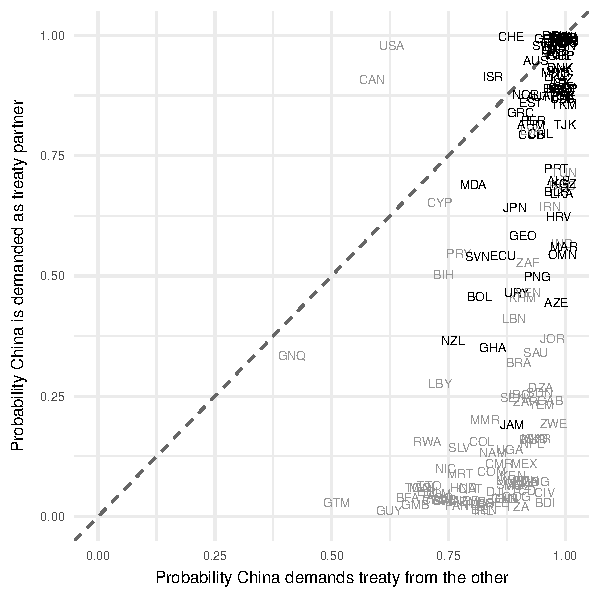
\includegraphics[width=.4\textwidth]{figure1_a.pdf} & 
		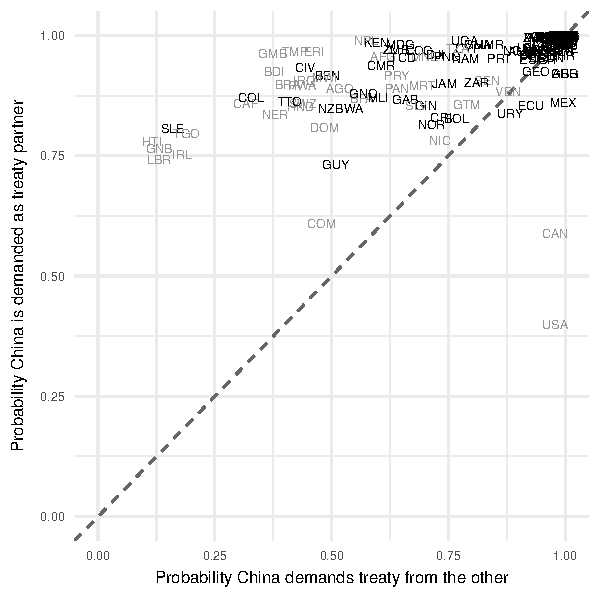
\includegraphics[width=.4\textwidth]{figure1_b.pdf} \\
	\end{tabular}
	\caption{Each panels displays the posterior mean probability that China demands and will be demanded as a BIT partner. Country labels in black designate those that had formed a BIT with China by the specified year.}	
	\label{fig:predplotCHN}
\end{figure}
\FloatBarrier

Figure~\ref{fig:predplotUSA} illustrates a different use of the P-GBME model.  It shows the predicted probabilities that the USA is demanded (left) and demands (right) a BIT in 2010.  Observe that the model predicts Peru, Mexico, and Chile---the top 3 non-BITs---demand a BIT with the USA at probabilities close to one, and are also likely BIT targets of the USA with probabilities exceeding $0.5$. Closer inspection of UN treaty data reveals that, by 2010, all three had signed other agreements with the US that contain provisions functionally equivalent to BITs; these agreements do not appear in the BIT dataset commonly used in the literature.\footnote{The treaties are 2006 Peru-USA Free Trade Agreement (FTA), NAFTA in 1992, and the 2003 Chile-USA FTA. These agreements included investment provisions that mirror the terms of a BIT almost exactly (see \url{http://investmentpolicyhub.unctad.org/Download/TreatyFile/5454}).} The P-GBME model nevertheless highlights these ``hidden'' agreements as dyads likely to have a BIT. This suggests that researchers studying BITs need to carefully examine the dataset they employ and perhaps expand the set of treaties considered relevant.

\begin{figure}[ht]
	\centering
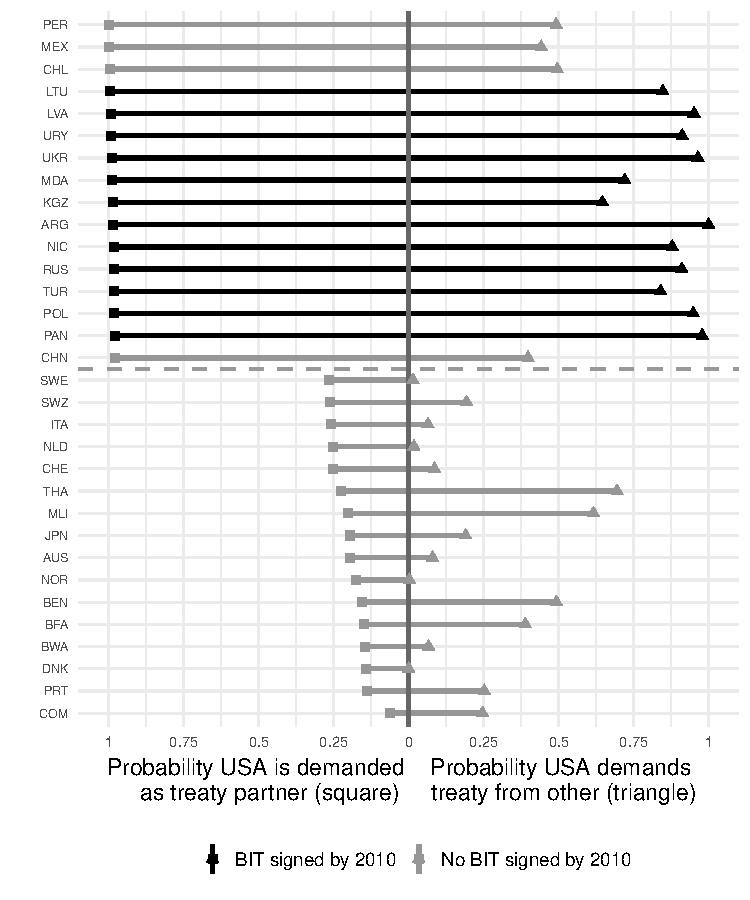
\includegraphics[width=.7\textwidth]{figure2.pdf} 
\caption{The posterior probability a country demands a BIT (left) and is demanded (right) with the USA in 2010 (the top and bottom decile of countries).  P-GBME is good at separating likely from unlikely treaties as well as identifying ``hidden agreements.''}	
	\label{fig:predplotUSA}
\end{figure}
\FloatBarrier
